%% Prepared for submission to SN Computer Science (Springer Nature).
%% Built on the official Springer Nature LaTeX authoring template
%% (sn-jnl.cls) with the sn-basic reference style and numbered
%% bracketed citations, per SN Computer Science's submission guidelines.
%% Migrated 2026-08-27 from the corrected manuscript/dke/main.tex (the
%% Data & Knowledge Engineering / elsarticle version); all scientific
%% corrections from that migration (Exact20 denominator, residual-error
%% decomposition, DeepOR/OR-R1 and OptMATH provenance wording, evaluation
%% dates, runtime/complexity, StrictInstantiationReady motivation) are
%% retained as migration history; metric definitions were revised 2026-10-27. See
%% docs/SNCS_STAGE3_MANUSCRIPT_SPRINGER_REPOSITORY_FINALIZATION_2026-08-27.md
%% for the full audit trail.

\documentclass[pdflatex,sn-basic,Numbered]{sn-jnl}

\usepackage{graphicx}
\usepackage{multirow}
\usepackage{amsmath,amssymb,amsfonts}
\usepackage{booktabs}
\usepackage{tabularx}
\usepackage{algorithm}
\usepackage{algorithmicx}
\usepackage{algpseudocode}
\usepackage{url}
\usepackage{xr-hyper}
\usepackage{hyperref}
% Avoid duplicate caption destinations in the preserved Springer template.
\hypersetup{hypertexnames=false}

\raggedbottom

\externaldocument[S-]{supplement}[Retrieval_Assisted_Scalar_Grounding_JDSA_Phase1_Supplement.pdf]
\begin{document}

\title[Retrieval-Assisted Scalar Grounding]{Retrieval-Assisted Scalar Grounding for Natural-Language Optimization: A Diagnostic Study}

\author*[1]{\fnm{Soroush} \sur{Vahidi}}\email{sv96@njit.edu \textnormal{(ORCID: 0000-0003-1934-6282)}}

\affil*[1]{\orgdiv{Department of Computer Science, Ying Wu College of Computing}, \orgname{New Jersey Institute of Technology}, \orgaddress{\street{University Heights}, \city{Newark}, \postcode{07102-1982}, \state{NJ}, \country{USA}}}

\abstract{Translating natural-language requirements into optimization models requires both selecting a mathematical structure and grounding its parameters in textual evidence. Strong retrieval or well-formed output alone cannot establish that these parameters express the intended problem. We investigate this distinction through a diagnostic evaluation that separates schema retrieval, scalar coverage and type checks, and numerical agreement across all required scalar parameters. On 331 NLP4LP queries and a fixed catalog of 335 schema documents, lexical and pretrained dense retrieval identify the target schema for 301 and 313 queries, respectively. However, ratio-aware lexical grounding passes the coarse readiness criterion on 265 queries (80.06\%), while only seven (2.11\%) meet the full stored-reference scalar-tolerance criterion. The evaluated pipeline uses reference-derived parameter inventories and query-reference scalar eligibility, so these results characterize assisted grounding rather than autonomous formulation. A separate study of Gemini, DeepSeek served through io.net, and Cohere covers 217 relationship judgments per model across 16 NL4Opt training problems. After historical recovery, 631 of 651 judgments are structurally valid; agreement on 197 complete cases yields Fleiss' $\kappa=0.371$, without establishing semantic accuracy. Twelve contrast pairs, validated by the author with language-model assistance, additionally illustrate distinctions that semantic evaluation must preserve, without supplying new provider-performance measurements. Together, the analyses show the need to evaluate retrieved structure, numerical completeness and semantic fidelity separately. The conclusions are limited to exposed catalogs, reference-assisted inputs and the available archived evidence.}

\keywords{natural language processing, optimization modeling, knowledge representation, information retrieval, semantic grounding, intelligent information systems}

\maketitle

\bmhead{Acknowledgements}

The author is deeply grateful to his mother for her continuous emotional support. The author gratefully acknowledges Professor Ioannis Koutis of the New Jersey Institute of Technology (NJIT) for his academic guidance, encouragement, and continued support. The author also thanks NJIT for providing access to the Wulver high-performance computing cluster, which supported the computational research.

Special thanks are extended to Anders Borum, the developer of \mbox{Secure ShellFish}, for generously providing complimentary lifetime access to the application. \mbox{Secure ShellFish} facilitated secure remote access to computational resources and supported the research and development workflow.

The author also appreciates research computing support provided through the Cohere Labs Catalyst Grant Program, Google Cloud Research Credits Program, and io.net. This acknowledgment recognizes support to the author's broader research activities; use of these credits for the experiments reported here has not been established.

\section{Introduction}

Natural-language descriptions are an important source of data for optimization-based decision support. They specify what can be produced, which resources are available, how costs are incurred and which outcomes should be preferred. Turning those descriptions into a mathematical model requires more than recognizing relevant concepts or extracting numbers: each quantity must be assigned to the right entity, unit and mathematical role. A capacity and a cost can share the same numerical value but belong in different parts of a model. Likewise, changing ``at most'' to ``at least'' preserves the number while reversing the constraint. Such distinctions determine whether a model represents the decision problem that an analyst intended.

Research on natural-language optimization has approached this translation through entity extraction, structured representations and the generation of formulations or solver code \cite{ramamonjison2022autoformulation,ramamonjison2023nl4opt,kadioglu2024ner4opt,ahmaditeshnizi2024optimus_icml}. The need to connect textual evidence to a structured representation also appears in schema and value grounding for database queries \cite{deng2021strug}. Recent text-to-optimization research explicitly distinguishes selecting a model structure from binding its data \cite{gao2026models}. The remaining evaluation question is therefore not simply whether grounding is difficult, but which measurements reveal its failures and which can conceal them. A retrieved template may be appropriate while its parameter assignments are wrong; a complete-looking mapping may satisfy type checks while misrepresenting a resource limit; and an executable program or a consensus label may still lack evidence of semantic correctness.

We study this question through \emph{retrieval-assisted scalar grounding}. A retriever selects a schema document from a fixed catalog, and a deterministic procedure extracts numerical mentions and assigns them to scalar parameter slots. The resulting partial mapping is an intermediate representation, not a complete optimization formulation. Lexical retrieval and a pretrained dense alternative make it possible to examine retrieval and grounding separately, while assignment controls examine how candidate evidence and search affect the result. These established components serve as inspectable instruments for evaluating the transition from textual data to a formal representation.

The evaluation setting is deliberately explicit about its assistance. The catalog is derived from the benchmark and contains all target schemas; it is not a test of generalization to unseen mathematical structures. The historical pipeline obtains parameter keys from reference-derived schema metadata, with a reference-record fallback, and filters participation using the query reference's numeric scalar keys before assignment. Although the numerical selector does not receive the reference magnitudes, the overall pipeline is not gold-free. Its measurements describe what happens when part of the required structure is already supplied, making it important to distinguish success at an intermediate check from agreement across the full reference scalar inventory.

Three questions organize the study. \textbf{RQ1:} How reliably can a relevant schema be retrieved in this known-catalog setting? \textbf{RQ2:} Why does successful retrieval or coarse readiness fail to ensure complete scalar agreement, and what do controlled assignment comparisons reveal about that gap? \textbf{RQ3:} What can structural validity, agreement and source-grounded relationship judgments establish about semantic interpretation? The third question separates observed model behavior from the reference evidence needed to assess correctness; it does not treat agreement as a substitute for that evidence.

The primary evaluation uses 331 queries from \textsc{NLP4LP} \cite{nlp4lp_dataset} and 335 schema documents. Term frequency--inverse document frequency (TF--IDF) retrieval identifies the target schema for $301/331$ queries ($90.94\%$), and pretrained BGE-M3 retrieval does so for $313/331$ ($94.56\%$). In the ratio-aware TF--IDF grounding configuration, $265/331$ queries ($80.06\%$) pass coarse readiness, but only $7/331$ ($2.11\%$) meet the stored-reference tolerance criterion for every required scalar. This separation is the central empirical finding: a favorable retrieval or readiness result does not certify a complete numerical mapping. Fixed-score assignment controls on a separate 49-query pilot further distinguish changes in slot assignments from aggregate whole-instance gains. Their scope is the retained candidates and scores, rather than an unrestricted test of better semantic representations. Imperfect references and missing original scalar mappings also limit interpretation of stored-reference agreement as source-level correctness.

A complementary historical study examines structured relationship judgments from Gemini, DeepSeek served through io.net, and Cohere. Each model judges the same 217 relationships drawn from 16 \textsc{NL4Opt} training problems. The recovered records support $631/651$ structurally valid judgments and Fleiss' $\kappa=0.371$ over 197 complete cases. These are validity and agreement measurements on relationships clustered within problems, not semantic-accuracy estimates or an independent model ranking. A separate common-18 formulation comparison provides limited execution and terminal-objective evidence under heterogeneous protocols. It cannot be combined with relationship labeling or scalar grounding into a single performance measure.

To make the semantic distinctions concrete, we additionally use a diagnostic set of 12 controlled pairs, comprising 24 samples across eight categories. Ten pairs change meaning and two preserve meaning through paraphrase. Their labels have been validated by the author through a documented review assisted by a language model; they are not independently blinded gold labels. The cases illustrate numerical bounds, units, roles, variable references, ratios, logical conditions and irrelevant information. They share generation lineage and recurring mathematical templates, and no provider pilot was executed on this set. Their contribution is to specify interpretable semantic probes, not to demonstrate new model-specific failures or explain causally the whole-instance grounding count.

The contributions are threefold:
\label{subsec:intro_contributions}
\begin{enumerate}
\item An empirical decomposition of fixed-catalog retrieval, coverage/type readiness and agreement across all required scalar parameters, with explicit input assistance and denominators. It exposes the distance between selecting a suitable structure and instantiating its numerical content.
\item Controlled assignment and archived-measurement analyses that separate candidate, scoring and search effects from changes caused by evaluation procedures. These analyses delimit what the retained grounding and execution records can support.
\item A complementary examination of real-model relationship validity and agreement, together with author-validated semantic contrast cases. This distinguishes observable output conformity from the reference evidence needed for correctness claims.
\end{enumerate}

The resulting contribution to data science is an evaluation methodology for assessing how textual evidence becomes a structured decision representation. It supports interpretable diagnosis and reproducible scrutiny of intermediate measurements, while retaining the limits imposed by benchmark exposure, reference assistance and incomplete archives. Section~\ref{sec:related_work} situates the study; Sections~\ref{sec:task} and~\ref{sec:methodology} define the task and protocol. Section~\ref{sec:experiments} presents the grounding diagnostics, Section~\ref{sec:llm} examines the separate large-language-model evidence, and Section~\ref{sec:discussion} discusses implications and limitations.

\section{Related Work}
\label{sec:related_work}

Recent advances in natural-language-to-optimization modeling reflect a shift from entity extraction to end-to-end generative systems, and increasingly to structured grounding and retrieval. We organize this literature around four primary axes that situate the present study.

\subsection{End-to-End LLM Optimization-Model Generation}
\label{subsec:rw_llm_generation}

End-to-end systems use LLMs to generate formulations or solver code, extending earlier entity and meaning-representation tasks such as NL4Opt \cite{ramamonjison2023nl4opt}. OptiMUS and OptLLM combine formulation, code generation and debugging \cite{ahmaditeshnizi2024optimus_icml,zhang2024optllm}. LLMOPT and ORLM study trained modeling systems \cite{jiang2025llmopt,huang2025orlm}; OptMATH develops synthetic optimization data \cite{lu2025optmath}. SIRL and OR-R1 use solver-informed learning \cite{chen2025solver,ding2026orr1}, while DeepOR studies a foundation model for optimization \cite{xiao2026deepor}. Agentic and experience-based approaches include OptimAI, AlphaOPT and ORThought \cite{thind2025optimai,kong2025alphaopt,yang2026orthought}. Their formulation or execution outcomes differ from this paper's conditional scalar-assignment diagnostics.

\subsection{Retrieval, Memory, and Solver-Feedback Systems}
\label{subsec:rw_retrieval_memory}

Retrieval and memory can augment generative modeling: OPT2CODE combines retrieval with code generation \cite{ahmed2025opt2code}; Autoformulation and uncertainty-aware approaches search over modeling decisions \cite{astorga2025autoformulation,yu2026uncertainty}. Chain-of-Experts coordinates specialized agents \cite{xiao2024chainofexperts}, while dual-cluster and experience-replay systems retain modeling or correction knowledge \cite{zhang2026dual,xie2026escaping}. Solver-independent formulation and question partitioning broaden the task further \cite{li2026solver,pan2025pamop}. These approaches generally use retrieval or feedback within open-ended generation; our catalog supplies the structure on which scalar assignment is conditioned.

\subsection{Binding and Structured Grounding}
\label{subsec:rw_binding}

As benchmarks mature, researchers have exposed a steep performance drop when transitioning from simple puzzles to complex formulations \cite{miplibnl2026}. This drop has motivated a critical distinction between a system's \emph{modeling} ability (selecting mathematical structure) and its \emph{binding} ability (grounding specific numeric parameters and data from text into that structure). Recent work by Gao et al.\ explicitly identifies data binding as a major limitation of generative text-to-optimization systems, reporting an effective binding limit in open-ended formulations \cite{gao2026models}. Earlier component-level approaches such as \textsc{Ner4Opt} \cite{kadioglu2024ner4opt} framed optimization modeling as an information-extraction problem over natural-language entities and quantities. Cross-domain text-to-SQL and schema matching provide related alignment settings \cite{yu2018spider,affolter2019nli,sheetrit2024rematch}. Formulation-equivalence checking addresses a further distinction: a program can execute successfully without expressing the intended optimization problem \cite{zhai2025equivamap}.

Our study addresses a narrower but complementary setting to the binding challenges identified by Gao et al.\ \cite{gao2026models}. We do not claim priority for the observation that binding is difficult. Their Text2Opt-Bench separates modeling from data binding as numerical scale grows. The July 2026 revision distinguishes oracle-fed BIND data externalization from a deployable trained binding specialist, and analyzes an untrained two-stage pipeline that fails to recover that benefit. Our narrower increment is the mismatch between assisted inventory/readiness gates and the all-key endpoint, together with frozen-objective and archival-measurement diagnostics. Our evidence concerns a different, already exposed benchmark and does not reproduce their scaling or intervention results. Rather than generating an open-ended formulation and then binding its data, we retrieve one schema from a fixed catalog and measure how retrieval errors alter the scalar slot inventory available to deterministic grounding---via oracle schema selection, StrictInstantiationReady, and an exhaustive residual-error decomposition.

Value grounding has related precedents outside optimization modeling. StruG learns column grounding, value grounding and column--value mapping for text-to-SQL \cite{deng2021strug}. Unit Dependency Graphs represent dependencies between quantities and units in arithmetic word problems \cite{roy2017udg}, while ILP-based semantic-role inference combines local evidence with linguistic constraints \cite{punyakanok2004ilp}. CQE represents quantities with units and associated concepts \cite{almasian2023cqe}. Execution-guided decoding rejects some faulty partial SQL programs \cite{wang2018execution}; successful execution still does not establish that an optimization model expresses its source problem. These connections motivate separate candidate, binding and consistency diagnostics; they do not validate the present heuristic or imply that it implements those systems. RAT-SQL explicitly learns schema relations and linking \cite{wang2020ratsql}, whereas PICARD constrains generated sequences through incremental parsing \cite{scholak2021picard}. These are precedents for structured alignment and output validity, not implementations or directly comparable baselines for our scalar-assignment task. In particular, a valid JSON judgment or executable program does not certify an occurrence--parameter relationship.

\subsection{Position of the Present Work}
\label{subsec:rw_position}

The present study isolates fixed-catalog retrieval and scalar assignment. Its lexical path is inference-time LLM-free, but its evaluated inputs remain reference-assisted. Table~\ref{S-tab:comparison_landscape} compares tasks rather than incomparable accuracy numbers; Section~\ref{subsec:exp_grounding_baselines} provides the matched conditional comparison. Maximum-sum one-to-one assignment is classical \cite{kuhn1955assignment}; the controlled decoder comparisons test its effect under frozen evidence, not a new matching algorithm.



\section{Task Definition and Evaluation Assumptions}
\label{sec:task}
\subsection{Problem Formulation}
\label{subsec:method_problem}

We study retrieval-assisted instantiation for natural-language optimization descriptions. Given a query, the system returns (i)~a top-1 schema from a fixed catalog and (ii)~scalar parameter assignments for that schema---an intermediate step before full model synthesis \cite{nlp4lp_dataset,ramamonjison2023nl4opt,ahmaditeshnizi2024optimus_icml}. Schema retrieval ranks $\mathcal{S}=\{s_1,\dots,s_M\}$ and returns
\begin{equation}
\hat{s}=\arg\max_{s \in \mathcal{S}} \mathrm{score}(q,s).
\label{eq:top1_schema}
\end{equation}
Parameter instantiation then extracts numeric mentions and assigns them to scalar slots of $\hat{s}$ with deterministic rules. Incorrect retrieval can mis-specify the eligible slot set even when the query contains usable numeric evidence.

A \emph{schema} here is the retrieved template together with its scalar parameter structure. The benchmarked setting does not synthesize a complete program, recover all variables/constraints, or reconstruct list-/vector-/dictionary-valued objects. Scope is restricted in three deliberate ways: (1)~scalar numeric parameters only; (2)~deterministic grounding (no generative LLM or learned extractor; no fine-tuning), with retrieval evaluated via lexical methods and pretrained BGE-M3; (3)~schema-conditioned scalar recovery rather than end-to-end generation. Proxy checks and gold-assisted reference-program execution later provide limited downstream diagnostics without redefining this core task (Section~\ref{subsec:exp_engineering}).

Let $K_G(q)$ contain keys whose gold values are numeric scalars (integers or floats, excluding booleans), and let $P_{\mathrm{all}}(\hat{s})$ contain \emph{all} keys in the predicted schema's parameter-metadata dictionary, falling back to all keys in its reference parameter record when the parameters metadata is not a dictionary. This original construction does not first select entries by scalar shape. The benchmark constructs assignments on the eligible set
\begin{equation}
E(q,\hat{s}) = K_G(q) \cap P_{\mathrm{all}}(\hat{s}),
\label{eq:eligible_slots}
\end{equation}
Thus gold scalar status filters the slot inventory \emph{before} assignment; gold keys affect both prediction construction and evaluation. Gold numerical magnitudes are not supplied to the mention-selection rule. Let $y_q : K_G(q) \to \mathbb{R}$ be the gold map and $\hat{y}_{q}$ the partial assignment on $A(q) \subseteq E(q,\hat{s})$; masked inputs may leave a raw unknown token rather than a numeric value. Retrieval quality is top-1 schema match; downstream quality is how well eligible scalars can be filled from text. As shown later, retrieval on \textsc{NLP4LP} is already strong, while residual difficulty concentrates in scalar grounding.

\subsection{Evaluation Inputs and Reference Assistance}
\label{subsec:assistance-setting}

Reference access must be distinguished from reference scoring. The main four-arm and matched-baseline experiments are \emph{gold-assisted}: the expected scalar count and slot identities depend on $K_G(q)$ before a value is chosen. Slot-name type heuristics consequently also operate on reference-derived names. The numeric selector does not receive the gold magnitudes, objective coefficients or constraint identities as separate targets; this narrower blindness does not make the complete pipeline autonomous.

The catalog itself is benchmark-derived. Its builder pairs each test description with the same record's parameterized description (falling back to its description and a metadata signature). The retained catalog contains 331 test-record documents plus four fillers; all 331 target IDs are present, and six query--target texts match exactly. This is a known-template identification setting, not a held-out template-generation test. Unsupervised fitting of an index is compatible with that setting, but does not establish independence from the evaluation source.

The later joint/factorial controls remove the query-specific gold-key filter, yet retain the selected reference template's slot names, shapes and descriptions, with types inferred heuristically from names. They remain \emph{partially assisted}; available parameter relations also come from that template. Their results measure assignment conditional on supplied structure. By contrast, the 20-case execution check additionally retains reference code and unfilled scalar/structured values and is gold-assisted. Supplement, Section~\ref{S-app:reproduction} identifies these boundaries and separates prediction reconstruction from aggregation. No autonomous formulation score, or adjustment estimating one from these conditional scores, is identifiable from the saved records.

\subsection{Inference Dependencies and Practical Scope}
\label{subsec:inference-dependencies}

The primary path uses a catalog-fitted TF--IDF representation, cosine ranking, numeric parsing and typed assignment. It calls no LLM and requires no task-specific neural training or LLM-generated relationship labels. Optional BGE-M3 retrieval does use a pretrained neural encoder. External generation baselines, the auxiliary annotation audit, and research/writing assistance use LLMs separately; the research workflow is not wholly LLM-free.

With dependencies and reference metadata cached, the lexical path runs locally without model-service calls or per-token API charges. These are implementation properties, not measured comparative cost, privacy or reliability benefits. Deterministic replay additionally requires the original ordering/environment; reference-assisted inputs still prevent interpreting this path as autonomous deployment.

\subsection{Metric Levels and Denominators}
\textit{Schema R@1} is $N^{-1}\sum_{i=1}^N H_i$, where $H_i=\mathbb{1}[\hat{s}_i=s_i^*]$ and $N=331$. For downstream metrics, write $E_i=E(q_i,\hat{s}_i)$ and let $A_i\subseteq E_i$ be the assigned slots. Let $T_i\subseteq A_i$ contain assignments accepted by the implemented coarse-type compatibility predicate. This is not literal type equality: an integer mention is accepted for a float slot, and integer or float mentions are accepted for currency slots, in addition to same-type matches. Expected slot types are inferred heuristically from names, not annotated semantic roles. Define
\begin{equation}
c_i=\begin{cases}|A_i|/|E_i|,& |E_i|>0,\\0,& |E_i|=0,\end{cases}
\qquad
\textit{Coverage}=\frac{1}{N}\sum_{i=1}^N c_i,
\label{eq:coverage}
\end{equation}
\begin{equation}
t_i=\begin{cases}|T_i|/|A_i|,& |A_i|>0,\\0,& |A_i|=0,\end{cases}
\qquad
\textit{TypeMatch}=\frac{1}{N}\sum_{i=1}^N t_i.
\label{eq:typematch}
\end{equation}
Both reported scores are \emph{macro-averages over queries}, including zero-denominator queries as zero. They are not pooled slot ratios. Separate type-stratified diagnostic files pool slots by type and therefore use a different aggregation. An abstention leaves a slot unfilled, reducing coverage; TypeMatch conditions on assigned slots within each query, then averages across all queries. Missing retrieval yields an empty eligible set and zero coverage and type score. A masked mention can count as assigned while lacking a comparable numerical value; the implemented unknown mention type does not pass the coarse-type predicate.

For a schema-hit query, let $C_i\subseteq A_i$ contain slots with both a numeric prediction and numeric gold value. For each comparable slot,
\begin{equation}
 e_{i,s}=\frac{|\hat{y}_{i,s}-y_{i,s}|}{\max(1.0,|y_{i,s}|)}.
\label{eq:bounded_error}
\end{equation}
A slot passes the inclusive tolerance rule if $e_{i,s}\leq0.20$: absolute error at most $0.20$ for $|y|<1$, otherwise relative error at most $20\%$. No additional type gate is imposed on this numerical comparison. With $J=\{i:H_i=1,\ |C_i|>0\}$,
\begin{equation}
x_i=\frac{1}{|C_i|}\sum_{s\in C_i}\mathbb{1}[e_{i,s}\leq0.20],
\qquad
\textit{Exact20 (on hits)}=\frac{1}{|J|}\sum_{i\in J}x_i.
\label{eq:exact20}
\end{equation}
The CSV field \texttt{exact20} stores $x_i$, a fraction of slots, not a whole-query indicator. It is blank on schema misses or when $C_i$ is empty. Such queries are excluded, rather than zero-filled, in the reported Exact20 mean; an empty $J$ is reported as unavailable. Main-table denominators are 291, 291, 303, and 320 \emph{queries} for TF--IDF baseline, TF--IDF ratio-aware, BGE-M3, and Oracle. Missing numerical predictions do not count as errors in this conditional metric, so abstention can improve Exact20 while lowering coverage. Its method-dependent subsets do not support an unconditional accuracy ranking.

\textit{InstantiationReady} retains its historical metric identifier for reproducibility and is described here as \emph{coarse readiness}:
\begin{equation}
\mathit{InstantiationReady}_i=\mathbb{1}[c_i\geq0.8\ \wedge\ t_i\geq0.8].
\label{eq:instantiation_ready}
\end{equation}
The reported score is its mean over all $N$ queries. It checks neither schema correctness nor numerical values, and can tolerate unfilled or incompatible slots. StrictInstantiationReady additionally requires $H_i=1$; it still does not check values.
\begin{equation}
\mathit{StrictInstantiationReady}_i = \mathbb{1}[H_i=1\ \wedge\ c_i\geq0.8\ \wedge\ t_i\geq0.8],
\label{eq:strict_instantiation_ready}
\end{equation} Empty eligible or assigned sets fail both readiness criteria. Thus an $80\%$ coarse-readiness rate is not an $80\%$ correct-instance rate.

\section{Methods and Experimental Protocol}
\label{sec:methodology}\label{sec:method}
\subsection{Retrieval-Based Schema Identification}
\label{subsec:method_retrieval}

The retriever ranks the 335 benchmark-derived schema descriptions and passes only its top-1 identifier downstream. This is known-template identification, not open-domain search or unseen-template induction. The selected template exposes parameter keys; Eq.~\eqref{eq:eligible_slots} then applies the benchmark's gold scalar filter.

We evaluate BM25 \cite{robertson2009bm25}, TF--IDF cosine retrieval \cite{pedregosa2011sklearn}, LSA \cite{deerwester1990lsa}, and pretrained dense BGE-M3 \cite{chen2024m3embedding} (Table~\ref{S-tab:retrieval_backbones}). Classical methods fit their unsupervised representations to the fixed catalog without query-label supervision; BGE-M3 is used off-the-shelf. No novel-schema generalization is evaluated. Equation~\eqref{eq:top1_schema} defines the selected schema; only that top-1 result is passed downstream. An \emph{oracle} control substitutes the gold schema to expose grounding under perfect retrieval. A \emph{random} reference is $1/335 \approx 0.0030$ for retrieval-only evaluation, or a uniformly chosen schema passed through the same grounding pipeline for downstream evaluation. Wrong retrieval can shrink or misalign the eligible slot set; strong retrieval supplies a more appropriate inventory for deterministic grounding.



\subsection{Deterministic Parameter Instantiation}
\label{subsec:method_instantiation}

Given a query and predicted schema, the second stage produces slot--value assignments for eligible scalar parameters. It does not generate a complete model or recover variables, constraints, or structured objects. A fixed rule-based extractor recognizes integers, decimals, written numbers, fraction words, percentages, currency-like forms, comma-separated magnitudes and the supported multiplicative ratio words; masked tokens in degraded settings are preserved as numerically unknown. Mentions receive a coarse type from \{\emph{percent}, \emph{integer}, \emph{currency}, \emph{float}\} via surface cues. Eligible slots are the intersection in Eq.~\eqref{eq:eligible_slots}; expected types are inferred from parameter names, and mention compatibility is defined below. This gold-assisted filtering is part of the evaluated protocol, rather than an independently inferred scalar inventory.

Typed greedy matching is the primary benchmark assignment rule. With eligible slots $\mathcal{P}=\{p_1,\dots,p_m\}$ and an indexed collection of mentions $\mathcal{T}=\{t_1,\dots,t_n\}$, where equal values at different source occurrences remain distinct mentions,
\begin{equation}
t_i^{*} = \arg\max_{t \in \mathcal{T}\setminus \mathcal{U}_{i-1}} \mathrm{compat}(p_i,t),
\label{eq:typed_assignment}
\end{equation}
where $\mathcal{U}_{i-1}$ are previously used mentions. Compatibility ranks coarse type preference, then absolute numeric magnitude, then raw surface text; remaining ties retain source order. Assigned mention indices are not reused, although equal values at other occurrences remain available. Slot order follows the recorded run's Python set iteration and is not portable without its interpreter/hash configuration. Section~\ref{subsec:exp_grounding_baselines} compares this rule to other already-implemented same-task alternatives under fixed TF--IDF retrieval (typed greedy and constrained assignment use distinct token/mention constructors with related ratio-aware patterns; others retain intrinsic enriched extractors). Typed greedy remains strongest on InstantiationReady / StrictInstantiationReady; some alternatives raise conditional Exact20 by abstaining more. A selective schema-and-grounding reranking diagnostic (not a grounding-only comparison) showed an apparent InstantiationReady gain driven by wrong-schema artifact (Section~\ref{subsec:exp_significance}). Algorithm~\ref{alg:instantiation} and Figure~\ref{fig:instantiation-pipeline} summarize the common backbone.

Optional lexicon-based role cues for tie-breaking exist but are not part of the primary main-benchmark configurations and carry no formal correctness guarantee. A numeric-extraction ablation adds supported multiplicative ratio-word values (e.g., ``twice'' becomes 2 and ``triple'' becomes 3); experiments show gains in TypeMatch and InstantiationReady with retrieval unchanged.

\begin{algorithm}[t]
\caption{Deterministic parameter instantiation: extract and type mentions; intersect predicted parameter keys with gold scalar keys; assign without token reuse under a deterministic compatibility rule.}
\label{alg:instantiation}
\small
\begin{algorithmic}[1]
\Require Query text $q$, predicted schema $\hat{s}$, gold scalar keys $K_G(q)$
\Ensure Slot--value mapping $A$
\State Extract numeric mentions $\mathcal{T}$ from $q$
\State Infer a coarse type for each mention in $\mathcal{T}$
\State Obtain parameter keys from schema $\hat{s}$
\State Set $\mathcal{P}=P_{\mathrm{all}}(\hat{s})\cap K_G(q)$; use the run's set iteration order
\State Infer an expected type for each slot in $\mathcal{P}$
\State Initialize assignments $A \leftarrow \emptyset$ and used-mention set $\mathcal{U}\leftarrow \emptyset$
\For{each slot $p_i \in \mathcal{P}$}
    \State Define candidate set $\mathcal{C}_i \leftarrow \mathcal{T} \setminus \mathcal{U}$
    \If{$\mathcal{C}_i = \emptyset$}
        \State \textbf{continue}
    \EndIf
    \State Score mentions in $\mathcal{C}_i$ using a deterministic slot--mention compatibility rule
    \State Select the highest-ranked mention $t_i^{*}$
    \State Assign $A[p_i] \leftarrow \mathrm{value}(t_i^{*})$ if numeric; otherwise retain its raw unknown token
    \State Update $\mathcal{U} \leftarrow \mathcal{U} \cup \{t_i^{*}\}$
\EndFor
\State \Return $A$
\end{algorithmic}
\end{algorithm}

\begin{figure}[t]
  \centering
  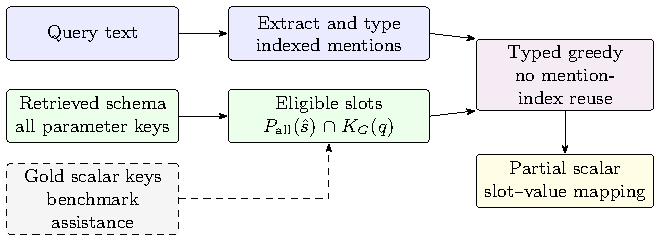
\includegraphics[width=0.98\linewidth]{figures/pipeline_m1.pdf}
  \caption{Schema-conditioned deterministic parameter instantiation. The query supplies typed numeric mentions. All predicted-schema metadata keys, with reference-key fallback, are intersected with gold scalar keys to form participating slots; this benchmark assistance is explicit. Assignment consumes mention indices, not unique numerical values. The diagram describes the historical typed-greedy protocol; the later metadata-only factorial protocol uses a different inventory.}
  \label{fig:instantiation-pipeline}
\end{figure}

\subsection{Evaluation-Oriented Design Choices}
\label{subsec:method_design}

Core metrics are solver-free. Reference-key filtering can let a wrong schema pass coverage/type gates on a small overlapping inventory; StrictInstantiationReady therefore adds schema match. Oracle selection is a control, not a formal upper bound on every metric. Neither readiness gate checks numerical values or complete-model correctness, and reference-program execution is evaluated separately.

\subsection{Experimental Setup}
\label{subsec:exp_setup}

We evaluate on \textsc{NLP4LP} \cite{nlp4lp_dataset,ahmaditeshnizi2024optimus_icml}, a curated gated public benchmark of LP/MILP descriptions pairing each instance with a gold parameter record and reference solver code. Unless noted, results use the 331-query test split; each query has one gold schema and is ranked against the 335-document catalog (random top-1 chance $1/335 \approx 0.0030$). These are historically designated test queries that have also been used repeatedly during development and retrospective analysis; the split name does not imply an untouched confirmatory evaluation. Three query variants probe robustness: \emph{orig} (full text), \emph{noisy} (controlled lexical corruption and numeric masking), and \emph{short} (first sentence only).

Retrieval uses BM25, TF--IDF, LSA, and off-the-shelf BGE-M3 (no benchmark fine-tuning); only top-1 schemas enter grounding, with an oracle control for perfect selection. Downstream grounding follows Section~\ref{subsec:method_instantiation}, restricted to scalar slots induced by the predicted schema. Reported configurations are: (i)~TF--IDF typed-greedy with baseline extraction; (ii)~TF--IDF typed-greedy with ratio-aware extraction; (iii)~BGE-M3 with the same ratio-aware grounding; (iv)~oracle typed-greedy. Configurations (ii) and (iii) use the same grounding implementation. However, their frozen assignments differ even on shared schema hits (Section~\ref{subsec:exp_error}); numerical differences cannot be attributed solely to retrieval.

Unless noted, retrieval and readiness metrics use the full denominator; Exact20 is the sole conditional exception. Paired significance uses the recorded resampling procedures with $B=10{,}000$ and seed $42$, plus exact McNemar tests where noted (Section~\ref{subsec:exp_significance}). We also report overlap sanitization diagnostics, the numeric-extraction ablation (Section~\ref{subsec:exp_error}), and three restricted structural/solver studies (Section~\ref{subsec:exp_engineering}). Table~\ref{S-tab:exp_blocks} summarizes blocks. Classical retrieval and grounding are CPU-compatible. BGE-M3 reporting metadata specifies float32 L2-normalized 1024-dimensional embeddings and cosine similarity, but does not authenticate the execution device or complete environment. Data/software references include Hugging Face \texttt{datasets} \cite{lhoest2021datasets} and \textsc{scikit-learn} \cite{pedregosa2011sklearn}.

The preserved headline CSVs contain query-level evaluation metrics, not scalar maps. They match their first committed versions and support reconstruction of the reported summary statistics, but the original per-instance scalar assignments were not retained in the inspected archival outputs and cannot be independently reevaluated. Separate cached controls do preserve actual choices. Supplement, Section~\ref{S-app:reproduction} distinguishes these evidence types; no newer predictions replace missing originals.



\section{Diagnostic Results}
\label{sec:experiments}
The central result is a separation between retrieving a suitable schema, filling its scalar inventory, and agreeing with every required stored-reference scalar. TF--IDF retrieves the target for $301/331$ queries, while its ratio-aware grounding passes coarse readiness on $265/331$ but complete scalar tolerance on only $7/331$. Alternative grounding pipelines raise the latter count to as many as $46/331$, even though their readiness rates are lower. Tables~\ref{tab:nlp4lp-grounding-baselines} and~\ref{tab:nlp4lp-error-taxonomy} show why both numerical completeness and failure-stage accounting are necessary. These are the reference-assisted, exposed-catalog diagnostics defined in Section~\ref{subsec:assistance-setting}, not autonomous formulation scores.

\subsection{Schema Retrieval Across Query Variants}
\label{subsec:exp_retrieval}
Within the fixed 335-document catalog, BGE-M3 retrieves the target for $313/331$ original queries ($94.56\%$), compared with TF--IDF's $301/331$ ($90.94\%$). The paired discordances are 15 BGE-only and three TF--IDF-only hits; the retrospective exact test gives unadjusted $p=0.0075$ and Holm-adjusted $p=0.0302$ in the stated family of 16 comparisons. Noisy-query retrieval remains close to the original-query rates, whereas first-sentence truncation reduces every method's accuracy (Table~\ref{tab:nlp4lp-retrieval-main}). Means across the three variants, computed before rounding, are $0.9013$ for BGE-M3, $0.8640$ for TF--IDF, $0.8469$ for BM25 and $0.8328$ for LSA. TF--IDF provides the primary lexical backbone; BGE-M3 tests whether the numerical failure boundary persists in a stronger-retrieval configuration.

\begin{table}[t]
  \centering
  \caption{Schema retrieval accuracy across query variants, reported as \textit{Schema R@1}. Each nonrandom value is reconstructed from saved top-1 schema IDs over all 331 test queries in the corresponding variant. The random baseline is the theoretical top-1 chance rate under uniform schema selection over the 335 candidate schemas, i.e., $1/335 \approx 0.0030$. Best result in each column is shown in bold.}
  \label{tab:nlp4lp-retrieval-main}
  \small
  \begin{tabular}{lcccc}
    \toprule
    Baseline & Orig & Noisy & Short & Avg. \\
    \midrule
    Random  & 0.0030 & 0.0030 & 0.0030 & 0.0030 \\
    LSA     & 0.8459 & 0.8882 & 0.7644 & 0.8328 \\
    BM25    & 0.8822 & 0.8912 & 0.7674 & 0.8469 \\
    TF--IDF & 0.9094 & 0.9033 & 0.7795 & 0.8640 \\
    BGE-M3 (dense) & \textbf{0.9456} & \textbf{0.9426} & \textbf{0.8157} & \textbf{0.9013} \\
    \bottomrule
  \end{tabular}
\end{table}
\subsection{Readiness Does Not Establish Complete Scalar Agreement}
\label{subsec:exp_downstream}
On the same 331 original queries, ratio-aware TF--IDF grounding passes ordinary readiness on 265 and schema-gated readiness on 255; ten wrong-schema cases pass the ordinary gate. Yet only seven cases satisfy complete stored-reference scalar tolerance. BGE-M3 and Oracle show the same separation: coarse readiness is $273/331$ and $281/331$, respectively, while complete scalar tolerance is $3/331$ and $8/331$. Correct retrieval and a nearly filled, type-compatible inventory therefore leave a substantial numerical validation problem.

Table~\ref{tab:nlp4lp-downstream-main} reports the previously defined diagnostics. Conditional Exact20 is higher for ratio-aware TF--IDF ($0.2614$) than for BGE-M3 ($0.2436$) or Oracle ($0.2505$), but its method-dependent comparable subsets cannot establish an unconditional accuracy ranking. Oracle supplies the correct schema to the same imperfect grounding procedure; it is a retrieval control, not an upper bound on a different grounding method.

\begin{table}[t]
  \centering
  \caption{Main downstream diagnostics on the original queries, computed from frozen evaluation records. InstReady and Strict measure coarse readiness without checking numerical values. \textit{Coverage}, \textit{TypeMatch}, \textit{InstantiationReady}, and \textit{StrictInstantiationReady} use the full 331-query denominator. \textit{Exact20} (on hits) is conditional on schema-hit cases with comparable predicted and gold numeric values. Best non-oracle result in each column is shown in bold.}
  \label{tab:nlp4lp-downstream-main}
  \small
  \setlength{\tabcolsep}{3.2pt}
  \renewcommand{\arraystretch}{1.12}
  \begin{tabular}{@{}lccccc@{}}
    \toprule
    Method & Coverage & TypeMatch & Exact20 & InstReady & Strict \\
    \midrule
% BEGIN GENERATED metric_audit_main_rows.tex
TFIDF-TG (baseline extr.) & 0.8794 & 0.8515 & 0.2449 & 0.7764 & 0.7462 \\
TFIDF-TG (ratio-aware extr.) & 0.8886 & 0.8665 & \textbf{0.2614} & 0.8006 & 0.7704 \\
BGE-M3 + ratio-aware & \textbf{0.9154} & \textbf{0.8946} & 0.2436 & \textbf{0.8248} & \textbf{0.8006} \\
Oracle-TG & 0.9416 & 0.9230 & 0.2505 & 0.8489 & 0.8489 \\
% END GENERATED metric_audit_main_rows.tex
    \bottomrule
  \end{tabular}

  \vspace{2mm}
  \raggedright
  \footnotesize
  TFIDF-TG denotes typed-greedy grounding; Oracle-TG uses the reference schema. Exact20 macro-averages the per-query slot fractions in Eq.~\eqref{eq:exact20} over 291, 291, 303 and 320 comparable schema-hit queries, respectively; noncomparable cases are excluded. All cells aggregate saved query metrics, not retained scalar mappings.
\end{table}
\subsection{Matched Grounding: More Complete Successes, Lower Readiness}
\label{subsec:exp_grounding_baselines}
Holding the query frame and TF--IDF retrieval fixed reveals improvements that a readiness-only comparison would miss. The full-gold-key tolerance counts are $7$, $40$, $37$, $35$, $46$ and $9$ out of 331 for typed greedy, constrained assignment, maximum-weight matching, optimization-role repair, search-structured grounding and semantic-IR repair, respectively (Table~\ref{tab:nlp4lp-grounding-baselines}). Search-structured grounding has the largest observed count, $46/331$ ($13.90\%$), while still failing this criterion on most queries. Constrained assignment gains 36 complete successes and loses three relative to typed greedy. Its historical eligible-only count is 41: query 102 fills three of seven required reference keys and is excluded from the all-key count of 40.

The direction reverses for coarse readiness. Typed greedy has the highest ordinary and Strict rates ($0.8006$ and $0.7704$); all five alternatives are lower, with Holm-adjusted $p\leq0.0059$ for the ten readiness comparisons. Some alternatives also increase conditional Exact20 while reducing coverage, so abstention and the conditional denominator matter. The all-key counts add the complementary requirement that every required scalar be present and pass tolerance; their descriptive ordering is not a multiplicity-adjusted superiority claim.

These are comparisons of complete grounding procedures. Candidate construction, context, scoring, abstention and decoding change together, and both typed greedy and constrained assignment already prevent mention reuse. The alternatives were selected before their matched scores were computed, with no additional tuning against the 331 labels for that comparison, but prior benchmark exposure remains. The observed numerical gains cannot be assigned solely to global search. Section~\ref{subsec:grounding-followup} examines the narrower question using fixed candidates and scores.

\begin{table}[t]
  \centering
  \caption{Matched same-task grounding baselines from saved metrics on the $331$ original queries with TF--IDF retrieval held fixed. Queries and retrieval are fixed under the gold-assisted inventory rule; candidate construction, context, scoring, abstention and decoding can differ. Best InstantiationReady / StrictInstantiationReady values are shown in bold. Full$_G$ requires the correct schema, all gold scalar keys, compatible types and complete stored-reference scalar tolerance; its denominator is 331 for every row.}
  \label{tab:nlp4lp-grounding-baselines}
  \scriptsize
  \setlength{\tabcolsep}{2.2pt}
  \renewcommand{\arraystretch}{1.12}
  \begin{tabular}{@{}lcccccc@{}}
    \toprule
    Grounding method & Coverage & TypeMatch & Exact20 & InstReady & Strict & Full$_G$ \\
    \midrule
    Typed greedy (reference) & 0.8886 & 0.8665 & 0.2614 & \textbf{0.8006} & \textbf{0.7704} & 7/331 \\
    Constrained assignment & 0.8531 & 0.8745 & 0.5772 & 0.7613 & 0.7311 & 40/331 \\
    Max-weight matching & 0.8436 & 0.8740 & 0.5225 & 0.7432 & 0.7130 & 37/331 \\
    Optimization-role repair & 0.8436 & 0.8724 & 0.5210 & 0.7372 & 0.7069 & 35/331 \\
    Search-structured grounding & 0.8195 & 0.8795 & 0.6397 & 0.7039 & 0.6737 & 46/331 \\
    Semantic-IR repair & 0.8131 & 0.8483 & 0.4949 & 0.7160 & 0.6949 & 9/331 \\
    \bottomrule
  \end{tabular}

  \vspace{2mm}
  \raggedright
  \footnotesize
  Typed greedy and constrained assignment share ratio-aware patterns but use different token/mention constructors and context. Their comparison changes scoring, abstention and decoding together; it does not isolate global search. The other rows use intrinsic enriched extractors as part of their grounding definitions. \textit{Exact20 (on hits)} denominators are 291 comparable schema-hit queries for all rows except semantic-IR repair (285), under the same exclude-noncomparable convention as Table~\ref{tab:nlp4lp-downstream-main}.
\end{table}
\subsection{The Dominant Residual Boundary Is Numerical Agreement}
\label{subsec:exp_error}
Table~\ref{tab:nlp4lp-error-taxonomy} partitions each configuration's 331 cases in order: schema miss, incomplete eligible coverage, incompatible types, stored-value disagreement, then full scalar-tolerance success. Missing numerical evidence never counts as success. In these original-query records, full assignment makes every eligible scalar comparable; every successful case in the four headline configurations also covers all reference scalar keys. The eligible-only exception for constrained assignment is disclosed above. ``Fully correct'' here denotes the scalar criterion in Eq.~\eqref{eq:bounded_error}, not exact equality, structured-parameter recovery or complete-model correctness.

For ratio-aware TF--IDF, the partition is $30+31+49+214+7=331$. Stored-value disagreement accounts for $214/331=64.65\%$ of all queries and $214/221=96.83\%$ of those passing correct-schema, full-coverage and full-type gates. BGE-M3 and Oracle likewise fail the value criterion on $228/231=98.70\%$ and $239/247=96.76\%$ of their respective gate-passing subsets. Thus the principal residual boundary is numerical agreement after the structural checks, although those method-specific subsets must not be treated as identical populations.

These partitions identify a failed evaluation stage, not the frequency of linguistic causes such as unit confusion or incorrect resource binding. Nor do the BGE-M3 differences isolate retrieval's effect: the two frozen configurations share 298 schema hits but differ in Exact20 on 162 of them. Historical slot iteration depends on Python set order; only TF--IDF records its hash seed. The missing BGE-M3 environment and original scalar maps prevent resolving the cause of those assignment differences. Supplement, Section~\ref{S-app:reproduction} records the reconstruction boundary.

\begin{table}[t]
  \centering
  \caption{Mutually exclusive residual partition reconstructed from saved query metrics on all 331 original queries per configuration. Categories apply in the stated order; full coverage and types mean $c_i=t_i=1$. Fully correct requires all eligible scalar values within the inclusive tolerance of Eq.~\eqref{eq:bounded_error}, and does not certify complete model correctness. TF--IDF columns differ only in extraction; numerical differences involving BGE-M3 are descriptive (see text).}
  \label{tab:nlp4lp-error-taxonomy}
  \small
  \setlength{\tabcolsep}{4pt}
  \begin{tabular}{lrrrr}
    \toprule
    Category & TF--IDF base & TF--IDF ratio & BGE-M3 & Oracle \\
    \midrule
    % BEGIN GENERATED metric_audit_residual_rows.tex
Wrong schema & 30 & 30 & 18 & 0 \\
Incomplete coverage & 48 & 31 & 33 & 35 \\
Type mismatch & 61 & 49 & 49 & 49 \\
Value inaccurate & 186 & 214 & 228 & 239 \\
Fully correct (scalar tolerance) & 6 & 7 & 3 & 8 \\
Total & 331 & 331 & 331 & 331 \\
% END GENERATED metric_audit_residual_rows.tex
    \bottomrule
  \end{tabular}
\end{table}
\subsection{What Fixed-Score Assignment and Search Controls Establish}
\label{subsec:grounding-followup}
A separate 49-query, 277-slot factorial holds candidate pools and edge-score matrices fixed within decoder comparisons. Under contextual scores and one-to-one assignment, greedy-to-exact decoding increases exact numerical slot counts from 106 to 136 for typed candidates and from 100 to 133 for rich candidates. However, full-tolerance successes remain $5/49$, with one gained and one lost query. Neither contextual decoder contrast survives the separate Holm family of 240 exploratory endpoint tests. With reusable mentions and additive scores, independent selection is already globally optimal. These controls isolate a decoding contrast within their supplied template structure; they do not explain the full historical 331-query improvement.

The earlier joint-grounding pilot likewise retains $3/49$ successes for both local and joint selection on its overlap-free slice. Among its original 50 cases, 32 admit a criterion-correct mapping in the common candidate pools, eight retain one in the beam's top ten, and three select it. Exact diagnosis finds 23 strict objective-preference failures and six correct/incorrect score ties among those 32 cases. Value/type-distinct exact enumeration on the same 49 primary queries leaves retention at $9/49$ and selected correctness at $3/49$. More exhaustive search and greater numerical diversity therefore supplied no observed whole-instance gain for these frozen objectives. This is a conditional negative result, not equivalence or a general failure of mathematical constraints.

Supplement, Sections~\ref{S-app:factorial-details}--\ref{S-app:reproduction}, retain all factorial cells, pruning stages, exact certificates, reference-convention sensitivity and population accounting. The 64 collected factorial cases comprise 49 primary, 12 development, one overlap-reconciliation and two reference-only cases. Excluding known-overlap query 291 from the primary comparisons does not remove earlier benchmark exposure.


\subsection{Extraction, Statistical Qualifications and Robustness}
\label{subsec:exp_significance}
The ratio-word extraction correction improves the coverage/type diagnostics while leaving retrieval unchanged (Table~\ref{tab:nlp4lp-prefix-postfix}). Strict readiness rises from $247/331$ to $255/331$, with eight gains and no losses; full scalar-tolerance success rises only from six to seven. The exact paired/group test for the Strict gain is $p=0.0078125$, adjusted to $0.0302$. This supports the specific extraction correction, while the residual partition shows how much numerical disagreement remains.

\begin{table}[t]
  \centering
  \caption{Numeric-extraction ablation on the original queries, comparing the baseline and ratio-aware extraction configurations of the TF--IDF typed-greedy method. The ratio-aware configuration corrects multiplicative ratio-word numeric expressions. The strict coarse-readiness count (of 331) rises from 247 to 255; $\Delta$ is ratio-aware minus baseline; see Section~\ref{subsec:exp_significance} for the significance test.}
  \label{tab:nlp4lp-prefix-postfix}
  \small
  \setlength{\tabcolsep}{4pt}
  \begin{tabular}{lccc}
    \toprule
    Metric & Baseline & Ratio-aware & $\Delta$ \\
    \midrule
% BEGIN GENERATED metric_audit_ablation_rows.tex
Coverage & 0.8794 & 0.8886 & +0.0091 \\
TypeMatch & 0.8515 & 0.8665 & +0.0150 \\
Exact20 (on hits) & 0.2449 & 0.2614 & +0.0165 \\
InstantiationReady & 0.7764 & 0.8006 & +0.0242 \\
StrictInstantiationReady & 0.7462 & 0.7704 & +0.0242 \\
% END GENERATED metric_audit_ablation_rows.tex
    \bottomrule
  \end{tabular}
\end{table}
All inferential comparisons are retrospective. Table~\ref{tab:nlp4lp-significance} uses saved paired gate records, the existing 327 delexicalized text groups, marginal 95\% group-percentile bootstrap intervals ($B=10{,}000$, NumPy seed 42), exact groupwise method-swap tests and Holm adjustment over 16 retrieval/readiness contrasts \cite{holm1979followup}. The family contains five main-table contrasts, the BGE-M3--TF--IDF retrieval contrast and ten ordinary/Strict contrasts against the five grounding alternatives. It is separate from the factorial's 240-test family. These corrections address the earlier statistical procedures; they do not create untouched observations or eliminate template dependence. Supplement, Section~\ref{S-app:statistical-history} preserves the procedural history.

\begin{table}[t]
\centering
\caption{Correction-only paired reanalysis of the saved 331-query gate records (327 text groups). Difference is the first configuration minus the second; CI is a marginal 95\% paired group-bootstrap interval. Exact p-values use groupwise method swaps; the final column adjusts the stated family of 16 tests. All comparisons are exploratory.}
\label{tab:nlp4lp-significance}
\scriptsize
\setlength{\tabcolsep}{2.3pt}
\begin{tabular}{@{}p{0.42\linewidth}cccc@{}}
\toprule
Comparison & Diff & 95\% CI & $p$ & Holm $p$\\
\midrule
% BEGIN CORRECTED SIGNIFICANCE
TFIDF ratio -- Oracle (coarse) & $-0.0483$ & $[-0.0751,-0.0240]$ & $<0.001$ & $0.0028$ \\
TFIDF ratio -- Oracle (Strict) & $-0.0785$ & $[-0.1108,-0.0486]$ & $<0.001$ & $<0.001$ \\
TFIDF ratio -- baseline (Strict) & $+0.0242$ & $[0.0091,0.0423]$ & $0.0078$ & $0.0302$ \\
BGE-M3 -- TFIDF ratio (coarse) & $+0.0242$ & $[0.0030,0.0455]$ & $0.0386$ & $0.0386$ \\
BGE-M3 -- TFIDF ratio (Strict) & $+0.0302$ & $[0.0091,0.0534]$ & $0.0129$ & $0.0302$ \\
% END CORRECTED SIGNIFICANCE
\bottomrule
\end{tabular}
\end{table}
The historical sanitization aggregates retain or improve retrieval after number/stopword removal (Supplementary Table~\ref{S-tab:nlp4lp-overlap}). Their 331-document diagnostic index excludes four fillers and document-ID tokens; it differs from the main index, while baseline LSA agrees at $0.8459$. Missing per-condition predictions limit this to aggregate-supported robustness, not proof that lexical shortcuts or benchmark exposure have been removed. The separate overlap stratification places 327/331 queries in the high-overlap bucket (TF--IDF R@1 $0.9174$); only four are in the medium bucket.

A selective schema-reranking diagnostic illustrates why the schema gate remains useful: ordinary readiness increases from $257/331$ to $265/331$, but six of the eight newly ready queries use an incorrect schema. The gate removes ten TF--IDF cases in both extraction configurations (Table~\ref{tab:strict-instready}); the ratio-aware TF--IDF--Oracle gap is $0.0483$ for ordinary readiness and $0.0785$ for Strict, with corrected adjusted $p=0.0028$ and $p<0.001$, respectively. Neither gate checks numerical values.

\begin{table}[t]
\centering
\caption{Sensitivity check: canonical \textit{InstantiationReady} versus the stricter \textit{StrictInstantiationReady} (Eq.~\eqref{eq:strict_instantiation_ready}), all 331 original queries, computed from saved per-query metric records. $\Delta$ is standard minus strict; $n_{\text{differ}}$ counts queries whose readiness label changes.}
\label{tab:strict-instready}
\small
\begin{tabular}{lcccc}
  \toprule
  Method & InstReady & StrictInstReady & $\Delta$ & $n_{\text{differ}}$ \\
  \midrule
% BEGIN GENERATED metric_audit_strict_rows.tex
TFIDF-TG (baseline) & 0.7764 & 0.7462 & 0.0302 & 10 \\
TFIDF-TG (ratio-aware) & 0.8006 & 0.7704 & 0.0302 & 10 \\
Oracle-TG & 0.8489 & 0.8489 & 0.0000 & 0 \\
% END GENERATED metric_audit_strict_rows.tex
  \bottomrule
\end{tabular}
\end{table}
\subsection{Restricted Execution and the Limits of the Core Findings}
\label{subsec:exp_engineering}
The historical 60- and 269-case studies measure coverage/type and rendered-template proxies using optimization-role relation repair. They do not establish numerical or formulation correctness. A distinct compatibility-filtered 20-case study reports reference-program execution through a SciPy HiGHS shim: TF--IDF and Oracle both execute at $0.95$, with solver-success rates $0.80$ and $0.75$. Unfilled scalar and structured values retain reference defaults; the one-case success difference is descriptive. Original subset manifests and per-case outcomes are unavailable, and shared examples show that the 60/269 samples cannot be assumed disjoint. Supplementary Tables~\ref{S-tab:eng-structural} and~\ref{S-tab:eng-solver}, and Section~\ref{S-app:restricted-details}, preserve all reported rates and exact proxy definitions.

\label{subsec:exp_runtime}
The lexical pipeline's historical $1.09$\,s timing for 331 queries is contextual, not a repeated efficiency benchmark; its complexity, $3.29$\,ms/query rate and approximately $198$\,MB peak memory are retained in Supplement, Section~\ref{S-app:runtime-details}. Earlier grounding variants, learning histories and auxiliary diagnostics are also preserved there and in the evidence register, rather than mixed with the current matched comparison.

\label{subsec:numerical-grounding-challenges}
The core findings establish a gap between retrieving structure, passing coarse checks and satisfying the complete scalar criterion. They do not identify source-semantic correctness. Occurrence-level ambiguity and weak supervision motivate the separate relationship investigation in Section~\ref{subsec:relationship-audit}; Supplement, Sections~\ref{S-app:occurrence-boundary} and~\ref{S-app:supervision-audit}, preserve that distinction. Section~\ref{sec:llm} next examines archived formulation and relationship evidence under their own populations and protocols.

\section{LLM-Based Comparative Evidence}
\label{sec:llm}
\subsection{Archived Formulations on a Shared Subset}
\label{subsec:exp_external}
The scalar-grounding system emits a partial mapping rather than a complete program. Its readiness and scalar metrics are therefore outside the formulation comparison in Table~\ref{tab:ext-outcomes}; Supplementary Table~\ref{S-tab:ext-context} describes the different tasks and implementations. These are 18 historically selected problems, not an independent benchmark or an equal-budget model contest.

\begin{table}[t]
\centering\small
\caption{Offline reaggregation of archived common-18 records. Every system attempted generation on the same 18 cases. Parse denotes a retained AMPL parse or Python code extraction; Run denotes successful process/solve completion. Obj. counts valid numerical text extractions among successful runs, and Ref. counts available reference objectives among those extractions. Agreement is conditional on classifiable executed reference comparisons. W/H means withheld for insufficient precision; N/A means an unavailable execution environment.}
\label{tab:ext-outcomes}
\setlength{\tabcolsep}{2.5pt}
\begin{tabular}{@{}lccccc@{}}
\toprule
System & Parse /18 & Run /18 & Obj./run & Ref./obj. & Agree./comp.\\
\midrule
PaMOP reconstruction & 13/18 & 13/18 & 13/13 & 11/13 & W/H\\
OptMATH adaptation & 18/18 & 15/18 & 15/15 & 15/15 & 11/15\\
ORLM adaptation & 18/18 & N/A & N/A & N/A & N/A\\
GPT-5.4 zero-shot & 18/18 & 16/18 & 16/16 & 16/16 & 12/16\\
\bottomrule
\end{tabular}
\end{table}

\subsection{Objective Extraction, Precision and Failure Accounting}
The fixed selection precedes the comparison outcomes and covers the same IDs in every row. Zero-shot GPT-5.4 uses the Azure OpenAI deployment returning \path{gpt-5.4-2026-03-05}, one generation at temperature 0, and direct Gurobi code. The project-maintained PaMOP reconstruction uses the same snapshot at temperature 0.2 with decomposition and at most five correction iterations; its actual executable path is AMPL/Gurobi, including one AMPL presolve-only success. The project-maintained OptMATH adaptation uses the released Qwen2.5-7B checkpoint at temperature 0.8, and the ORLM adaptation uses its released LLaMA-3-8B checkpoint with greedy decoding. Different prompts, framing, weights, correction budgets and solver interfaces preclude a model or provider ranking.

The original Python execution harness selected the first objective-like string, which could be a heuristic incumbent. The correction instead requires a terminal optimal solver summary and checks it against the final standalone objective printed by the generated program. The original generated code, stdout and reference objectives are preserved; no program or model is rerun. Nine stored objective fields differ from these terminal values, and seven agreement labels change. All 31 successful Python runs have a valid terminal/printed objective pair. The corrected agreement counts are $11/15$ for adapted OptMATH and $12/16$ for zero-shot GPT-5.4, with four disagreements in each conditional set.

For continuity the reported Python proxy retains its original predicate. Let $a=\operatorname{round}_{\mathrm{even}}(\hat z)$ and $b=\operatorname{round}_{\mathrm{even}}(z^*)$, using Python's float conversion and nearest-integer ties-to-even behavior. Agreement is
\begin{equation}
 \mathbb{1}\!\left[\begin{cases}|a-b|\leq0.05,&b=0,\\ |a-b|/|b|\leq0.05,&b\ne0.\end{cases}\right].
 \label{eq:common18-objective-proxy}
\end{equation}
Full available numerical tokens are retained before that explicit comparison step. A separately recorded unrounded sensitivity uses absolute $0.05$ at a zero reference and relative $0.05$ otherwise; it gives identical classifications on these 31 cases. This agreement does not validate rounding for other objectives or make the systems' protocols identical.

PaMOP's historical absolute-$10^{-6}$ objective comparison has a different precision problem. Common-18 case 254 displays $16666.7$ although its solver summary prints $16666.66667$ against reference $16666.666666666664$. Even the latter text cannot certify that tolerance. More generally, the retained displayed equality does not establish an unrounded return at $10^{-6}$. We therefore withhold its aggregate objective-agreement score. Among 11 executed cases with numerical references, two discrepancies exceed a conservative last-displayed-unit uncertainty bound and nine remain precision-unresolved; two other executed cases have no reference objective. An algebraic witness for case 254 is documented separately and is not substituted as a recovered numerical solver result. No revised exact-agreement fraction is inferred.

Five PaMOP cases finish with parse failure; nine of its 13 successful cases execute without correction and four after correction. Adapted OptMATH has three unsuccessful processes, and zero-shot has two. Four of these five Python failures (cases 219 and 237 for both systems) invoke Gurobi, terminate infeasible or infeasible-or-unbounded, and then fail accessing an objective; OptMATH case 232 has a distinct nonlinear-constraint API construction error. These stages are not interchangeable semantic diagnoses. All successful runs report optimal/solved generated-model outcomes, with conditional feasibility counts $13/13$, $15/15$ and $16/16$ for PaMOP, OptMATH and zero-shot, respectively. This does not show that the generated models express the source problems.

ORLM has code extracted on all 18 cases but no execution because \path{coptpy} is unavailable. Its execution and objective columns remain N/A. The supplement gives each case's outcome, source/configuration identities and precision disposition. Missing rendered historical prompts and incompletely authenticated environments still limit exact generation replay. Objective agreement and successful execution do not establish formulation equivalence; the core scalar-grounding method remains outside these columns.

\subsection{Real-Model Judgments of Occurrence--Parameter Relationships}
\label{subsec:relationship-audit}
Retrieving a suitable schema leaves open which source occurrence expresses each parameter. We therefore examine whether actual LLM services give complete, structurally grounded and mutually consistent judgments on proposed occurrence--declaration relationships. This is a separate annotation/QC question from both the 331-query scalar-grounding study and the common-18 formulation comparison. It tests neither the autonomous correctness of the retrieval system nor accuracy against human labels.

The frozen October 27, 2026 records contain 217 distinct relationship items from 16 NL4Opt training problems \cite{ramamonjison2023nl4opt}, drawn as a category-covering, high-risk convenience packet from a previously inspected 100-problem review frame. They are not 217 independent problems, repeated independent trials, or a random corpus sample. Multiple relationships share problem text, numerical occurrences and declarations. Each service originally received 33 batches of up to eight targets, with complete source text, supplied variables, objective and constraints; peer judgments were withheld. The four nominal decisions are \texttt{CORRECT}, \texttt{INCORRECT}, \texttt{AMBIGUOUS} and \texttt{CANNOT\_DETERMINE}. These are model assertions, not verified truth labels. Each object must also supply an explanation, literal source quotations, valid source identifiers, omission notes, a shared-mention flag and uncertainty.

The requested models are \path{gemini-3.1-pro-preview} through Google Vertex AI, \path{deepseek-ai/DeepSeek-V4-Pro-0813} through io.net io.intelligence (recorded FP8), and \path{command-a-reasoning-08-2025} through Cohere's direct v2 API. DeepSeek here names the served model, not a direct DeepSeek API. All use temperature 0 and a 12,000-output-token cap; Gemini uses LOW thinking, Cohere a 256-token thinking budget, and io.net its default reasoning behavior. Sampling/analysis seed 20261027 is not an inference seed. The identifiers authenticate the requested or echoed service names, not underlying weight checksums or every server default.

\begin{table}[htbp]\centering\small
\caption{Structural validity on the same 217 relationship targets per service. Final counts combine original-valid objects, deterministic offline repairs and historically generated valid replacements under a revised format. They are not single-pass or equal-treatment accuracy estimates. No new calls were made for this revision.}\label{tab:relationship-validity}
\setlength{\tabcolsep}{3.5pt}
\begin{tabular}{@{}lrrrr@{}}\toprule
Service/model family & Original valid & Offline repairs & Valid replacements & Final valid\\\midrule
Vertex AI/Gemini & 215 & 2 & 0 & 217/217\\
io.net/DeepSeek & 180 & 33 & 4 & 217/217\\
Cohere/Command A & 105 & 24 & 68 & 197/217\\\midrule
Total & 500 & 59 & 72 & 631/651\\\bottomrule
\end{tabular}\end{table}

Strict output-contract checks require exact source quotations and membership in supplied variable/formulation identifiers, in addition to JSON structure. Recovery v2.1 preserves all 500 originally valid objects, extracts only unique complete envelopes, maps only explicitly documented source aliases and losslessly serializes structured omission notes. Of 92 model-item targets still invalid after offline repair, historical smaller-batch requests with explicit identifier/quotation instructions yield 72 valid replacements. Cohere additionally uses a native JSON Schema with identifier enums; an initial rejected schema and a corrected transport are retained in the lineage. These changes affect comparability. The remaining 20 invalid Cohere objects all contain nonliteral evidence quotations; invalidity does not prove a mathematically wrong decision.

Among jointly valid pairs, nominal agreement is Gemini--DeepSeek $213/217$ ($98.16\%$), Gemini--Cohere $123/197$ ($62.44\%$), and DeepSeek--Cohere $120/197$ ($60.91\%$). The complete three-model denominator is 197, comprising 119 determinate unanimous cases, 77 disagreements and one unresolved case. The remaining 20 of 217 are invalid/incomplete. The unresolved case has three \texttt{CORRECT} labels but no verified lexical endpoint, so raw label unanimity is $120/197$, while determinate unanimity is $119/197$. Neither is semantic accuracy.

Fleiss' nominal $\kappa$ on the 197 complete cases is $0.370807$ (observed pair agreement $0.739425$, chance term $0.585858$), using all four decision categories and excluding invalid objects rather than coding them as an opinion. The complete-case marginal counts are 420 \texttt{CORRECT}, 168 \texttt{INCORRECT}, two \texttt{CANNOT\_DETERMINE} and one \texttt{AMBIGUOUS}, totaling 591 judgments. Original complete cases number only 89, with $\kappa=0.501643$; those same 89 cases retain identical labels after recovery. The change in aggregate $\kappa$ reflects expanded complete-case membership, not measured loss or gain in correctness. We report no population confidence interval, significance claim or model ranking for these clustered, selected items.

Verifiable defects include a singular variable alias rejected against a plural source identifier, prose/structured-note output that violates the schema, and quotations that paraphrase rather than copy the source. Valid decisions also differ on source-occurrence binding: Supplement, Section~\ref{S-app:relationship-evidence} gives identified witnesses and the per-problem denominator ledger. These examples explain protocol failures or conflicting model assertions, not independently adjudicated semantic error frequencies. No human-verified reference judgments exist for the 217 targets, and no consensus is approved as training gold. The study complements the retrieval/readiness gap: a retrieved template and a plausible structured judgment can both look usable while correct source binding remains unverified. Agreement cannot validate the retrieval pipeline's autonomous performance.


\section{External Validation, Discussion, and Limitations}
\label{sec:discussion}
\subsection{External Component-Level Robustness Validation}
\label{subsec:exp_external_validation}

As a component-level check, we evaluated numeric extraction on a fixed 1,000-instance \textsc{OptMATH}-Train sample \cite{lu2025optmath} (no fixed schema catalog, so extraction only). Pooled raw AST code-value overlap recall is $0.7501$; pooled automatic text-support recall is $0.8118$ (complete-instance rate $0.5910$). A secondary rule-based classifier on 150 instances (seed 20260815) estimates that $7.28\%$ of its inspected AST-value denominator are implementation, loop or solver constants. The later verification summary reports audit-calibrated text-supported recall as the pooled (micro) ratio $23{,}241/28{,}799=0.8070$ (95\% instance-bootstrap CI $[0.7842,0.8283]$, $B=10{,}000$, seed 42, over the 1,000 sampled instances). Its corrected per-instance counts are unavailable for independent rebootstrap of that historical CI. The reported mean of per-instance ratios (macro recall) is $0.8135$. The stored verification JSON reverses the names of these two aggregates; the values are preserved here with their implemented definitions. The 28,799 values are not independent samples, and occurrence-aware recall is not identifiable from these set-based artifacts. Two independently coded classifiers agree on $98.04\%$ of 4,801 literals in the 150-instance sample---automated cross-validation, not human gold labels. This is limited evidence that extraction transfers beyond \textsc{NLP4LP}; it does not establish full-framework generalization.

\subsection{Limitations and Threats to Validity}
\label{subsec:limitations}

\emph{Conditional task and imperfect references.} Main grounding uses gold scalar-key eligibility; later controls still receive reference template metadata. Neither demonstrates autonomous inventory discovery or complete formulation generation. Readiness omits value checks, while the full scalar criterion omits structured objects and model equivalence. Metadata may omit keys (query 102 exposes 3 of 7; query 293 has no eligible slots); successful cases in each of the four headline configurations cover all gold scalar keys, and the constrained eligible-only exception is disclosed separately. Stored references are not uniformly source-correct. The separate overlay in Supplement, Section~\ref{S-app:reference-conventions} is not maintainer-certified gold, and absolute 0.20 tolerance for fractions can accept materially different proportions.

\emph{Prediction retention and replay.} The inspected historical headline writers saved 13 metric columns, not scalar maps. The archival investigation authenticated the four metric CSVs, but found no matching assignment exports; deletion is not established. Stage-A, later cached choices and unverified archival candidates cannot replace them. Missing values and slot order prevent corrected-reference headline evaluation. BGE-M3's hash seed and complete execution environment are unrecorded; reporting metadata is not a runtime receipt. The three aggregate-supported tables and the extended subset study lack original per-condition or membership/outcome records (Supplement, Section~\ref{S-app:reproduction}). Gated dataset access also limits external reproduction.

\emph{Dependence and statistical scope.} The main experiments reuse one benchmark and a catalog constructed from its source records. Sanitization does not establish template independence; only four queries occupy the medium-overlap bucket. Grouping and the exclusion of query 291 address known text dependence but do not certify a fresh test set, independent templates or generalization across domains/languages. Earlier learned splits contain confirmed group crossings. Paired and factorial analyses are exploratory; multiplicity adjustments do not remove prior benchmark exposure. The selected 60/269/20 and common-18 studies support neither population-wide inference nor a harmonized end-to-end comparison.

\emph{Semantic supervision.} No formal independently accepted human reference set exists. The selected NL4Opt relationship audit in Section~\ref{subsec:relationship-audit} measures output structure and inter-model agreement, not semantic accuracy. Its recovery stages use different output-format instructions and incomplete-case selection changes the agreement population. It neither evaluates the 331-query pipeline nor supplies accepted training labels. Equality-derived weak labels, valid JSON, LLM consensus and source-semantic correctness are distinct. The targeted NL4Opt packet cannot estimate corpus-wide accuracy or exhaustive relationship recall, and its 713-problem source audit is not 713 certified independent training examples. Quarantine is precautionary; unflagged problems remain uncertified. Heuristic type/role cues have no correctness guarantee, and the residual partition cannot establish frequencies of particular semantic mechanisms.

\emph{Operational claims.} API-free lexical processing is an implementation property; comparative monetary cost, privacy, reliability and usability were not measured. BGE-M3 uses neural inference. The historical single-run timing and extraction-only OptMATH check do not establish production performance or full-framework transfer. No deployed-system or user study was conducted.
\subsection{Future Research Directions}
\label{subsec:future_work}

A possible future prerequisite is independent human validation of occurrence--parameter relations under a frozen rubric and sampling frame. A separate first-round protocol prepares 36 probability-sampled and 12 targeted relationships, with two overlaps (46 distinct cases across 16 problems); it has not yet produced formal reference labels. Its inferential scope is the selected 217-item frame, not the whole NL4Opt corpus. Source-reference and template-independence review must accompany any future use as supervision. This addresses a measured evidentiary gap before another scorer or encoder comparison is justified. Structured parameters and broader solver-backed validation remain outside the present claims. No new experiment or training run was performed for this revision.



\subsection{Closed Feasibility and Identifiability Audits}
\label{subsec:closed-audits}
Three closed audits clarify the information boundary without adding predictions. G1 found no validated autonomous slot-discovery/eligibility path in the current system. G2 found that the native gold operation selects participating slots, so removing a supposed numerical-candidate filter at fixed required slots is either vacuous or changes the task. G3 instead compared participation sets using saved TF--IDF schema IDs and metadata scalars with \texttt{shape=[]}. Sets are equal in 301/331 cases and differ in 30/331, adding 134 slot occurrences; 172/1,847 reference scalar occurrences are absent from predicted scalar inventories. Of the changed cases, 29 miss required reference keys under both conditions and one has no numeric scalar reference. Thus no informative whole-instance contrast is identified by those records. These are static methodological findings, not measured performance differences or tests of equivalence. Strict scalar metadata also changes the original all-key/fallback construction in seven cases, so the two inventory definitions cannot be silently substituted. Detailed set accounting is in the supplement. No further experiment was launched.
\section{Conclusion}
\label{sec:conclusion}
Retrieval accuracy, coverage/type readiness, numerical slot agreement and complete scalar agreement answer different questions. On the historical TF--IDF ratio-aware configuration, 265/331 queries (80.06\%) pass coarse readiness, 255/331 pass its schema-gated version, and only 7/331 (2.11\%) satisfy the full stored-reference scalar-tolerance criterion. All of these results condition on reference-derived participation and benchmark templates; none measures autonomous optimization.

Fixed-score assignment and exact-search diagnostics constrain claims about stronger decoding on the retained pilot, without establishing general equivalence. The corrected common-18 records support conditional terminal-objective proxy agreement of $11/15$ for adapted OptMATH and $12/16$ for zero-shot GPT-5.4. The PaMOP objective aggregate is withheld because archived precision is insufficient, while ORLM execution remains unavailable. These are evidence-qualified outcomes of heterogeneous formulation systems, not a capability ranking. The separate Gemini--DeepSeek--Cohere relationship audit exposes a complementary supervision boundary: 631/651 final objects pass the output contract, yet complete-case agreement ($\kappa=0.371$ on 197 relationships) supplies no human semantic truth. Its selected, clustered frame and targeted recovery preclude provider rankings or general accuracy claims. The contribution is an evidence-qualified diagnostic and reproducibility account, not a new retrieval/matching algorithm, a provider ranking, or a claim that numerical binding difficulty is newly discovered.
\backmatter

\section*{Declarations}

\noindent\textbf{Funding.} This research did not receive any specific grant from funding agencies in the public, commercial, or not-for-profit sectors. The external large-language-model baseline experiments used Microsoft Azure OpenAI services; associated usage was supported by the standard Azure for Students educational credit available to the author. NJIT/Wulver infrastructure access and complimentary Secure ShellFish access were institutional and in-kind assistance. The archived relationship-labeling runs identify providers but do not establish which research-credit awards paid for their use.

\noindent\textbf{Competing interests.} The author declares that there are no known competing financial interests or personal relationships that could have appeared to influence the work reported in this paper.

\noindent\textbf{Ethics approval and consent to participate.} Not applicable; this study did not involve human participants, human data, or animals. No formal human-annotation study contributes reference labels; the future validation protocol has not been carried out.

\noindent\textbf{Author contributions.} Soroush Vahidi: Conceptualization, Methodology, Software, Validation, Formal analysis, Investigation, Data curation, Writing -- original draft, Writing -- review \& editing, Visualization. This single-author paper uses the standard CRediT taxonomy to describe the contributions of the sole author.

\noindent\textbf{Data availability.} Historical derived metrics are public at \url{https://huggingface.co/datasets/SoroushVahidi/nl-optimization-instantiation-metrics}, under their existing CC BY-NC-SA 4.0 license. NLP4LP is obtained separately from \texttt{udell-lab/NLP4LP}; its current public card identifies CC BY-NC 4.0 and gated access. We provide upstream access instructions rather than redistribute that local cache. OptMATH raw data have an unresolved dataset license and are likewise obtained upstream. The MIT-licensed NL4Opt source subset, relationship prompts, per-case judgments, validity calculations and recovery lineage are prepared in a separate local release candidate, with account identifiers removed from copies. This M5 candidate is prepared for author inspection and has not been uploaded. Supplement, Section~\ref{S-app:reproduction} distinguishes directly verifiable results from missing historical predictions.

\noindent\textbf{Code availability.} Historical code is public at \url{https://github.com/SoroushVahidi/combinatorial-opt-agent}. The local M5 candidate adds deterministic verification entry points, manifests, source hashes and corrected evaluators. Its file-level inventory records included artifacts, sanitized derivatives, original licenses and concrete exclusions; preparation does not imply public availability of this revision.

\noindent\textbf{Reproducibility.} This revision uses frozen records and adds no model inference, solver execution or performance experiment. Released query metrics support aggregate checks; archived formulation logs support conditional objective comparisons; archived relationship responses support independent structure/agreement checks. Missing original headline scalar mappings, subset manifests, some rendered prompts and full-precision PaMOP returns prevent complete historical replay. Provider serving defaults and weight bytes are not fully authenticated. Compiling the source package reproduces the document, not missing measurements.

\noindent\textbf{Declaration of generative AI and AI-assisted technologies in the writing process.} During preparation the author used ChatGPT and Gemini to improve readability and language. OpenAI Codex later assisted manuscript revisions, evidence organization and deterministic validation. The author reviewed and edited the original work and remains responsible for its content; the M5 candidate awaits independent author review.

\noindent\textbf{Declaration of AI assistance in software development.} The author used Claude, Cursor and GitHub Copilot for coding assistance and reviewed, verified, tested and edited the resulting code. OpenAI Codex later assisted code corrections and offline verification scripts. The author retains responsibility for the implementation and reported results. Scientific LLM calls are identified separately; the evaluated scalar-grounding procedure uses no generative LLM inference.

\bibliography{references}

\end{document}
